%% Created by Yasuyuki SAITO, Department of Information Engineering.


%% 2016/01/13 Edit by Kouta ASAI, and Akira NEMOTO, Advanced Control and Information Engineering Course
%% 2017/12/07 Edit by by Shinichi OEDA, Department of Information Engineering.
%% 「★」マークが変更を加えた部分を表す

%% ★jsarticleに変更 fleqnで数式を左寄せにする
\documentclass[twocolumn, fleqn, uplatex]{jsarticle}

\usepackage{proceeding-DJ}
\usepackage{afterpage}
%% ★数式を使う人が多いと思うので
\usepackage{amsmath}
\usepackage{bm}
\usepackage{booktabs}
\usepackage{enumitem}
\usepackage{subcaption}


%% ★ヒラギノを使っている人向け
\usepackage[deluxe, expert]{otf}

% \makeatletter
% \long\def\@makecaption#1#2{%
%   \vskip\abovecaptionskip
%   \iftdir\sbox\@tempboxa{#1\hskip1zw#2}%
%     \else\sbox\@tempboxa{#1~ #2}%
%   \fi
%   \ifdim \wd\@tempboxa >\hsize
%     \iftdir #1\hskip1zw#2\relax\par
%     \else #1~ #2\relax\par\fi
%   \else
%   \global \@minipagefalse
%   \hbox to\hsize{\hfil\box\@tempboxa\hfil}%
% \fi
% \vskip\belowcaptionskip}
% \makeatother

\begin{document}

\pagestyle{empty}

%% 番号をつけるときはこのすぐ下の行を有効にして,番号を編集する.
%%\date{J--33}
%%所属をDJ以外にしたい場合は,styファイルを編集する.
\date{}
\titleJ{秘密分散法構築におけるユーザフレンドリーなUIの提案・評価・考察}
\titleE{Proposal, Evaluation and Discussion of user-friendly UI for Secret Sharing scheme construction}
\authorJ{三浦 夢生}
\authorE{Yu Miura}
\abstract{In modern society, spreads cloud or online service and a lot of important information (e.g. personal data) is transmitted and received.
Cyber-attacks against companies and organizations are increasing year by year, and the damage caused by ransomware, one of them, is expanding.
In this study, I deals with a scheme called secret sharing.
By using this scheme, we can reduce the risk of loss or theft of the secret. and allows managers to adjust discretion per role by using hierarchical one.
The purpose is designing intuitive and user-friendly UI for people who don't know too much about secret sharing and proposing easy to use secret sharing tool even individuals.
In an evaluation, I ask testers to use the proposed UI and the conventional CLI-based UI, and conduct a questionnaire survey and analysis of whether the UI is "visually easy to understand", "easy to operate", and "time required to build a secret sharing system".
}
% \keywords{The key word1 of the test for \LaTeXe \ template file, The key
% word2 of the test for \LaTeXe \ template file, The key word3 of the test
% for \LaTeXe \ template file}
\keywords{Secret Sharing, cryptgraphy, Shamir's Secret Sharing, User Interface}
\maketitle

%% 現在ページの上部へのフロートの配置を抑制.
%% ここに記述しておくことで,最初のページの左段上部に図表を置かない.
\suppressfloats[t]

\section{まえがき}
近年,クラウド及びオンラインサービスが%
企業や一般家庭において広く普及し\cite{lit:soumu-1},\cite{lit:soumu-2},%
個人情報などの多くの重要な情報がやり取りされている.%
その中で企業・団体等に対するサイバー攻撃は年々増加しており,%
その中の一つであるランサムウェアによる被害は拡大している\cite{lit:keisatu}.%
IPAの情報セキュリティ10大脅威においても,機密情報を狙った攻撃は%
大きな影響を与えるとされる\cite{lit:ipasec-1}.%
これらは機密情報やアクセス権の集中管理によって攻撃を受けた際のリスクが%
高まるためであり,最小限の適切なアクセス管理が重要である.%
しかし,無闇な機密情報のコピーや,アクセス権限の厳重化では%
かえってリスクが高まる\cite{lit:ipasec-2}.%

これらのリスク低減のため機密情報の分散管理及びアクセス権限の柔軟な付与が%
できる「秘密分散\cite{lit:nishikawa}」という技術を用いる.%
秘密分散によって情報の漏洩・紛失のリスクを低減し,%
またこれを階層化することによって管理者の役割ごとの裁量を調節できる手法を%
UIのバックエンドに採用する.%
フロントエンドサイドでは,秘密分散を詳しく知らないユーザでも%
直感的に利用しやすいUIの設計をする.%
本研究では個人で気軽に利用できるような秘密分散ツールの設計・提案を行い,%
UIによってどの程度秘密分散ツールが利用しやすくなったかアンケート調査し,%
提案UIの有用性や改善点について考察することを目的とする.

実装には,ユーザの環境を選ばずブラウザで動作するJavascriptと,%
そのフレームワークであるReact.jsを主として用いる.%
React.jsはGUI作成に特化したJavascriptフレームワークであり,%
SPA(Single Page Application)を作成しやすい画面遷移のない実装が可能となり,%
ユーザ側での画面読み込みや通信負荷を減らすことができる.%

アンケート調査ではコマンドラインライクなUIと木構造を模した提案UIを用意し,
それぞれファイルを秘密分散する課題を遂行してもらい,%
それにかかった時間の計測,使用感に関する質問への回答を求める.

\section{前提知識}
\subsection{Shamirの秘密分散法}
秘密分散法とは,まず対象となる秘密情報をあるアルゴリズムを用いて%
シェアと呼ばれる分散情報を作成し,%
そのシェアを管理する人・端末に配布し管理・保管する手法である.%
元の秘密情報を得る際には,管理されたシェアを必要な数だけ集め,%
復元アルゴリズムによって復元する.

いくつかある秘密分散法のうち,本研究ではShamirの秘密分散法\cite{lit:shamir}を用いている.%
この手法は$(k,n)$しきい値秘密分散法とも呼ばれ,シェアを$n$個生成し,%
$k$個のシェアを集めることで秘密情報の復元が可能であるが,%
$(k-1)$個以下のシェアからは復元は不可能である.

シェアを生成するアルゴリズムは,まずEq.\ref{randompoly}のような%
秘密情報$S$を定数項とするランダムな$k-1$次多項式を定める.
%
\begin{equation}
f(x) = S + a_{1}x + a_{2}x^{2} + \dots + a_{k-1}x^{k-1} \label{randompoly}
\end{equation}
%
管理に参加する人や端末の数$i$に対し,%
$f(1),f(2),\dots,f(i)$を計算し,配布する.

復元の際は,$k$個のシェア$(j,f(j))$を集めて$k$個の式を立て,%
連立方程式を解くことで秘密情報$S$を得る.
$k$個のシェアは同じ多項式から生成されたものであればよく,%
任意のものを用いればよい.

またこのときラグランジュ補間を用い,Eq.\ref{lagrange-1},Eq.\ref{lagrange-2}%
において$x=0$の場合を計算することで,多項式のうち定数項のみ,%
つまり元の秘密情報を得ることができる.
%
\begin{equation}
L(x) = \sum_{i=0}^{k}y_{i}l_{i}(x) \label{lagrange-1}
\end{equation}
%
\begin{equation}
l_{i}(x) = \prod_{j=0,j{\neq}i}^{k}{\frac{x-x_{j}}{x_{i}-x_{j}}} \label{lagrange-2}
\end{equation}
%
\section{提案UI}
本研究では感覚的に階層化された秘密分散法を構築できるGUIを提案する.%
階層化された秘密分散において,各階層の分散情報を頂点とし,%
分散情報と,その上位の分散情報を線で結び,%
それを辺とおくことで木構造として表現できる.
このとき,元となる機密情報を最上位ノードとし,%
それから生成された分散情報を子ノード,%
その各分散情報から生成された分散情報を子孫ノードとして定義し,%
パラメータ設定及び描画を行う.

\section{実装}
ブラウザ上で動作するアプリケーションによって,%
ユーザフレンドリーの環境に依存せず動作する実装を行う.
各ノードを,ノード名.パラメータ・子ノードを持つオブジェクトとして定義する.

\begin{figure}[htbp]
	\centering
	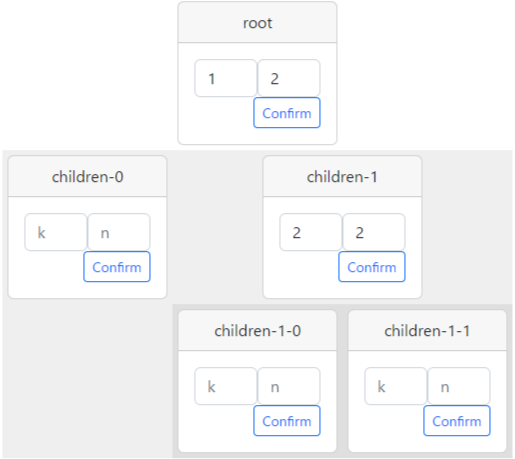
\includegraphics[width=5cm]{treeUI.png}
		\caption{Tree structure type UI.}
		\label{fig:treeUI}
\end{figure}

\begin{figure}[htbp]
	\centering
	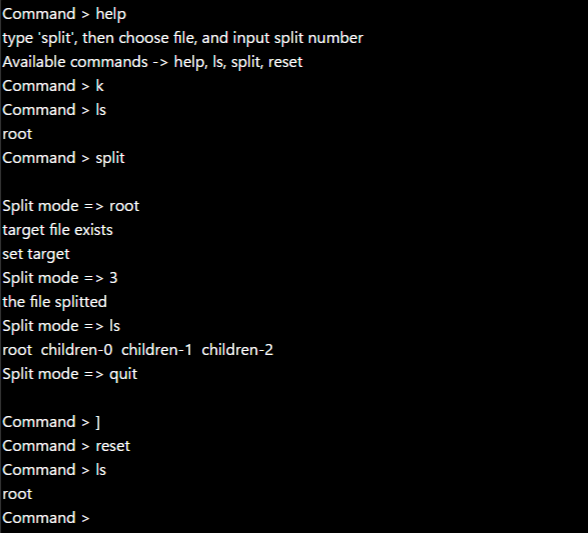
\includegraphics[width=5cm]{cliUI.png}
		\caption{CLI type UI.}
		\label{fig:cliUI}
\end{figure}

Fig.\ref{fig:treeUI}のように,初期状態から存在する最上位ノードに%
パラメータを入力し,分散情報を表す子ノードを動的に生成する.
同時に木構造全体の状態を保持するオブジェクトが更新され,%
そのオブジェクトを参照し,再帰的に木構造を描画する.

\section{アンケート調査}
アンケート調査は提案するUIと比較するため,%
Fig.\ref{fig:cliUI}に示すようなコマンドラインを模したUIを用意した.
アンケートの内容は,概要を説明できるほど秘密分散を知っているか,%
UIの使用感,秘密分散を施すイメージを掴めたか,%
実用を想定した際に選択肢の一つとなるか,その他感じたことについて回答を求めた.
実験参加者には①秘密分散・評価項目・UIのを説明を行い,%
②GUI,CUIの順にデモンストレーションを交えて説明し,%
③同様の順でそれぞれのUIを用いた課題に取り組み,%
④それぞれのUIに関するアンケートへの回答を求めた.%
②③④におけるUIの提示順は,参加者を二つのグループに分け一方はGUI,CUIの順,他方はCUI,GUIの順にすることでカウンターバランスを取った.

\section{結果・考察}
参加者6名に回答を求め,得られた結果の平均値をTable.\ref{tab:result}に示す.
評点は1~5の5段階で,数字が大きいほどポジティブなイメージを示す.%
6名全員が秘密分散の概要を知らなかった.

\begin{table}[htbp]
	\centering
	\caption{Average of survey results.}
	\label{tab:result}
	\scalebox{0.75}{
		\begin{tabular}{|c|c|c|}
		\hline
		& 木構造型UI & コマンドライン型UI \\
		\hline \hline
		\begin{tabular}{c}
		秘密分散のイメージが \\
		しやすいか
		\end{tabular} & 3.5 & 3.3 \\
		\hline
		使いやすいか & 4.3 & 3.5 \\
		\hline
		\begin{tabular}{c}
		実用を想定した際に \\
		選択肢となるか
		\end{tabular} & 4.3 & 3.3 \\
		\hline
		\end{tabular}
	}
\end{table}

全体として木構造型UIにおける平均値が高い結果となったが,%
イメージのしやすさはほとんど変わらなかった.%
これは事前説明の段階で秘密分散の概要を説明し,%
デモンストレーションを交えながら実際にその過程を見せたことで,%
その差がなくなったと考える.
使いやすさに関して,

\section{まとめ}
\section{今後の展望}

\begin{thebibliography}{9}
	\footnotesize
	\bibitem{lit:soumu-1}
		総務省, 
		``デジタルで支える暮らしと経済'', 
		情報通信白書, pp.156-159, July 2020.

	\bibitem{lit:soumu-2}
		総務省, 
		``デジタルで支える暮らしと経済'', 
		情報通信白書, pp.313-315, July 2020.
	
	\bibitem{lit:keisatu}
		警察庁, 
		``令和3年におけるサイバー空間をめぐる脅威の情勢等について'', 
		警察庁 広報資料, pp.3-5, April 2022.
	
	\bibitem{lit:ipasec-1}
		独立行政法人情報処理推進機構セキュリティセンター, 
		``情報セキュリティ10大脅威'', 
		情報処理推進機構, pp.36-39, March 2022.

	\bibitem{lit:ipasec-2}
		独立行政法人情報処理推進機構, 
		``組織における内部不正防止ガイドライン'', 
		情報処理推進機構, pp.40-44, April 2022.
	
	\bibitem{lit:nishikawa}
		西川律子,
		``秘密分散法の概要'', 
		沖テクニカルレビュー 第205号, pp.70-71, January 2006.

	\bibitem{lit:ipa}
		独立行政法人情報処理推進機構, 
		``企業における営業秘密に関する実態調査2020'', 
		調査実態報告書, pp.44-47, March 2020.
	
	\bibitem{lit:maruhi}
		株式会社エスロジカル, 
		``マル秘分散'', 
		http://www.ma-bu.com/, 
		閲覧日Dec 2021.
	
	\bibitem{lit:ssss}
		Jon Frisby, 
		``ssss'', 
		https://github.com/MrJoy/ssss, 
		閲覧日Dec 2021.
	
	\bibitem{lit:shamir}
		A Shamir, 
		``How to share a secret'', 
		Communications of ACM, Vol.22, pp.612-613, April 1979.
	
	\bibitem{lit:nozaki-1}
		野崎昭宏, 
		``納得する群・環・体'', 
		講談社, 第1版, pp.136-137, May 2016.
	
	\bibitem{lit:siozaki}
		汐崎陽, 
		``情報・符号理論の基礎'', 
		オーム社, 第2版, pp.90-91, May 2019.
	
	\bibitem{lit:nozaki-2}
		野崎昭宏, 
		``納得する群・環・体'', 
		講談社, 第1版, pp.160-176, May 2016.

	\bibitem{lit:takaara}
		高荒亮, 岩村惠一, 
		``XORを用いた高速な$(k,L,n)$ランプ型秘密分散法に関する研究'', 
		コンピュータセキュリティシンポジウム2009(CS2009)論文集, Vol.2009, pp.1-6, October 2011.
	
	\bibitem{lit:aono}
		青野成俊, 岩村惠一, 
		``実用観点からみた秘密分散法に関する一考察'', 
		コンピュータセキュリティシンポジウム2009(CS2009)論文集, Vol.2009, pp.1-6, October 2011.

\end{thebibliography}

\end{document}
